\section{Finden von Dokumenten mit ähnlichen Inhalten (Duplikaten Findung)}
\label{sec:FindenvonDokumenten}

%% Review on the different esb white papers to demonstrate that there is no mysql support through the esb for incomming connections, and the same for dynamic routing
In this section we discuss about the different approaches \ac{ESB} vendors take into account when accessing or storing data in \ac{SQL} database systems, and compare it to the support we provide in this work. 
Most of the \ac{ESB} vendors provide support for data persistency in \ac{RDBMS}. However, it is restricted to output connections to \ac{DBMS}. Fuse \ac{ESB} provides \ac{JDBC} data source support, enabling users to connect to a database and make \ac{SQL} based queries and updates \cite{FuseIntro}. This connection can be established during routing, when receiving a JMS or HTTP message in a consumer endpoint, etc. However, they do not provide support for native database communication protocol incoming messages, e.g. MySQL or PostgreSQL communication protocol. Thus, data consumer endpoints supporting native database protocols are not deployable. The same limited support is provided in the integration framework Camel, in its component Camel-jdbc \cite{cameljdbc}.

 \begin{figure}[htb]
	\centering
		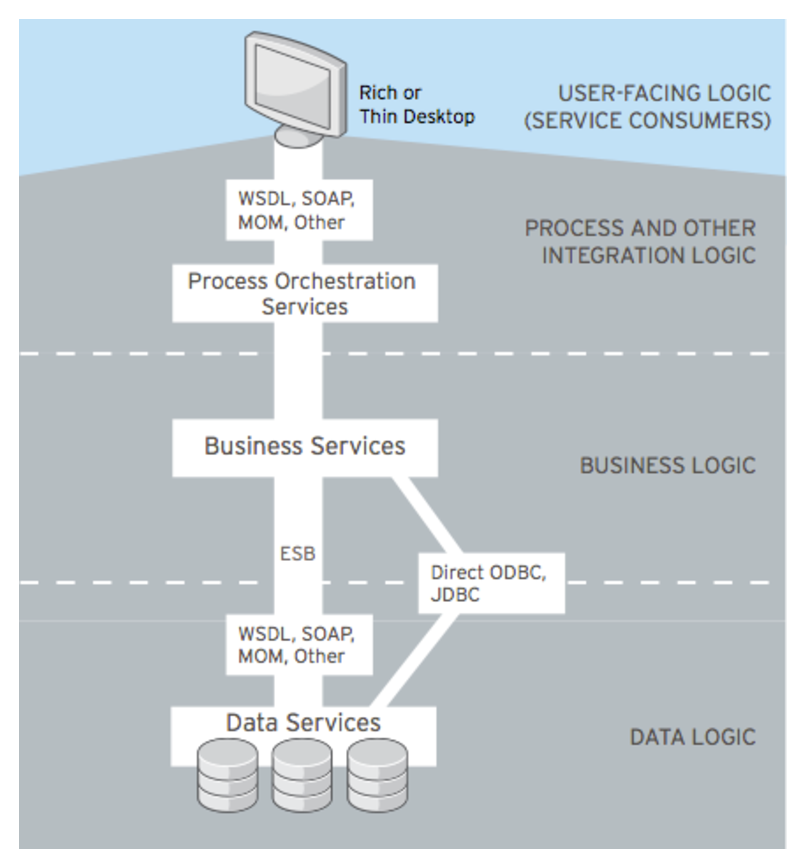
\includegraphics[clip, scale=0.4]{./gfx/jbossds.pdf}
	\caption[JBoss SOA and Data Services Integration]{JBoss Enterprise Data Services Platform \cite{jboss2011}}
	\label{fig:jbossdataservice}
\end{figure}

JBoss presents its Enterprise Data Service Platform containing data services with \ac{SOA} support, and an \ac{ESB} \cite{jboss2011}. Any organization currently using an \ac{ESB} can interoperate their Data Services Platform through open standards \cite{jboss2011}. Accessing the database layer using methods which implement the \ac{SOA}, e.g. Web services, requires the application to support such methods. One of the main goals in this diploma thesis is to minimize the adaptations in the DAL when migrating the data to the Cloud. Furthermore, as we can see in Figure \ref{fig:jbossdataservice}, connection utilizing native database protocol is established directly from the business application logic to the data service. In our approach we propose a native database connection through the \ac{ESB} to the data service. 